%%%%%%%%%%%%%%%%%%%%%%%%%%%%%%%%%%%%%%%%%%%%%%%%%%%%%%%%%%%%%%%%%%%%%%%%
%
%  AAMAS-2027 submission -- "Contagion"
%
%  PAGE LIMIT (per the Call for Papers): the main track is AT MOST 8 PAGES of
%  content; pages containing bibliographic references are additional and
%  unlimited. Keep the body within 8 pages. Subsections marked
%  "% CUT-CANDIDATE" are the first candidates to trim if it overruns.
%
%  TO COMPILE YOU NEED: aamas.cls (from the AAMAS-2027 template package /
%  Overleaf), the ACM CC-BY image file `by`, and the .png figures in this
%  directory. The `by` file ships with the template package, not with this
%  repository, so a missing-`by` error is expected until the template is in
%  place.
%
%%%%%%%%%%%%%%%%%%%%%%%%%%%%%%%%%%%%%%%%%%%%%%%%%%%%%%%%%%%%%%%%%%%%%%%%

%%% LaTeX Template for AAMAS-2027 (based on sigconf.tex)
%%% Prepared by the AAMAS-2027 Publication Chairs based on the version from AAMAS-2026.

%%% == IMPORTANT ==
%%% For anonymized submission, use this
\documentclass[sigconf,anonymous]{aamas}

%%%% For camera-ready, use this
% \documentclass[sigconf]{aamas}

%%% Load required packages here (note that many are included already).
%%% NOTE: `aamas' (like acmart) already loads amsmath, amssymb and booktabs, so
%%% reloading them here causes "Command \Bbbk already defined". Only the extra
%%% packages we actually need are loaded.
\usepackage{balance}   % for balancing columns on the final page

%%%%%%%%%%%%%%%%%%%%%%%%%%%%%%%%%%%%%%%%%%%%%%%%%%%%%%%%%%%%%%%%%%%%%%%%

%%% AAMAS-2027 copyright block (do not change!)

\makeatletter
\gdef\@copyrightpermission{
  \begin{minipage}{0.2\columnwidth}
   \href{https://creativecommons.org/licenses/by/4.0/}{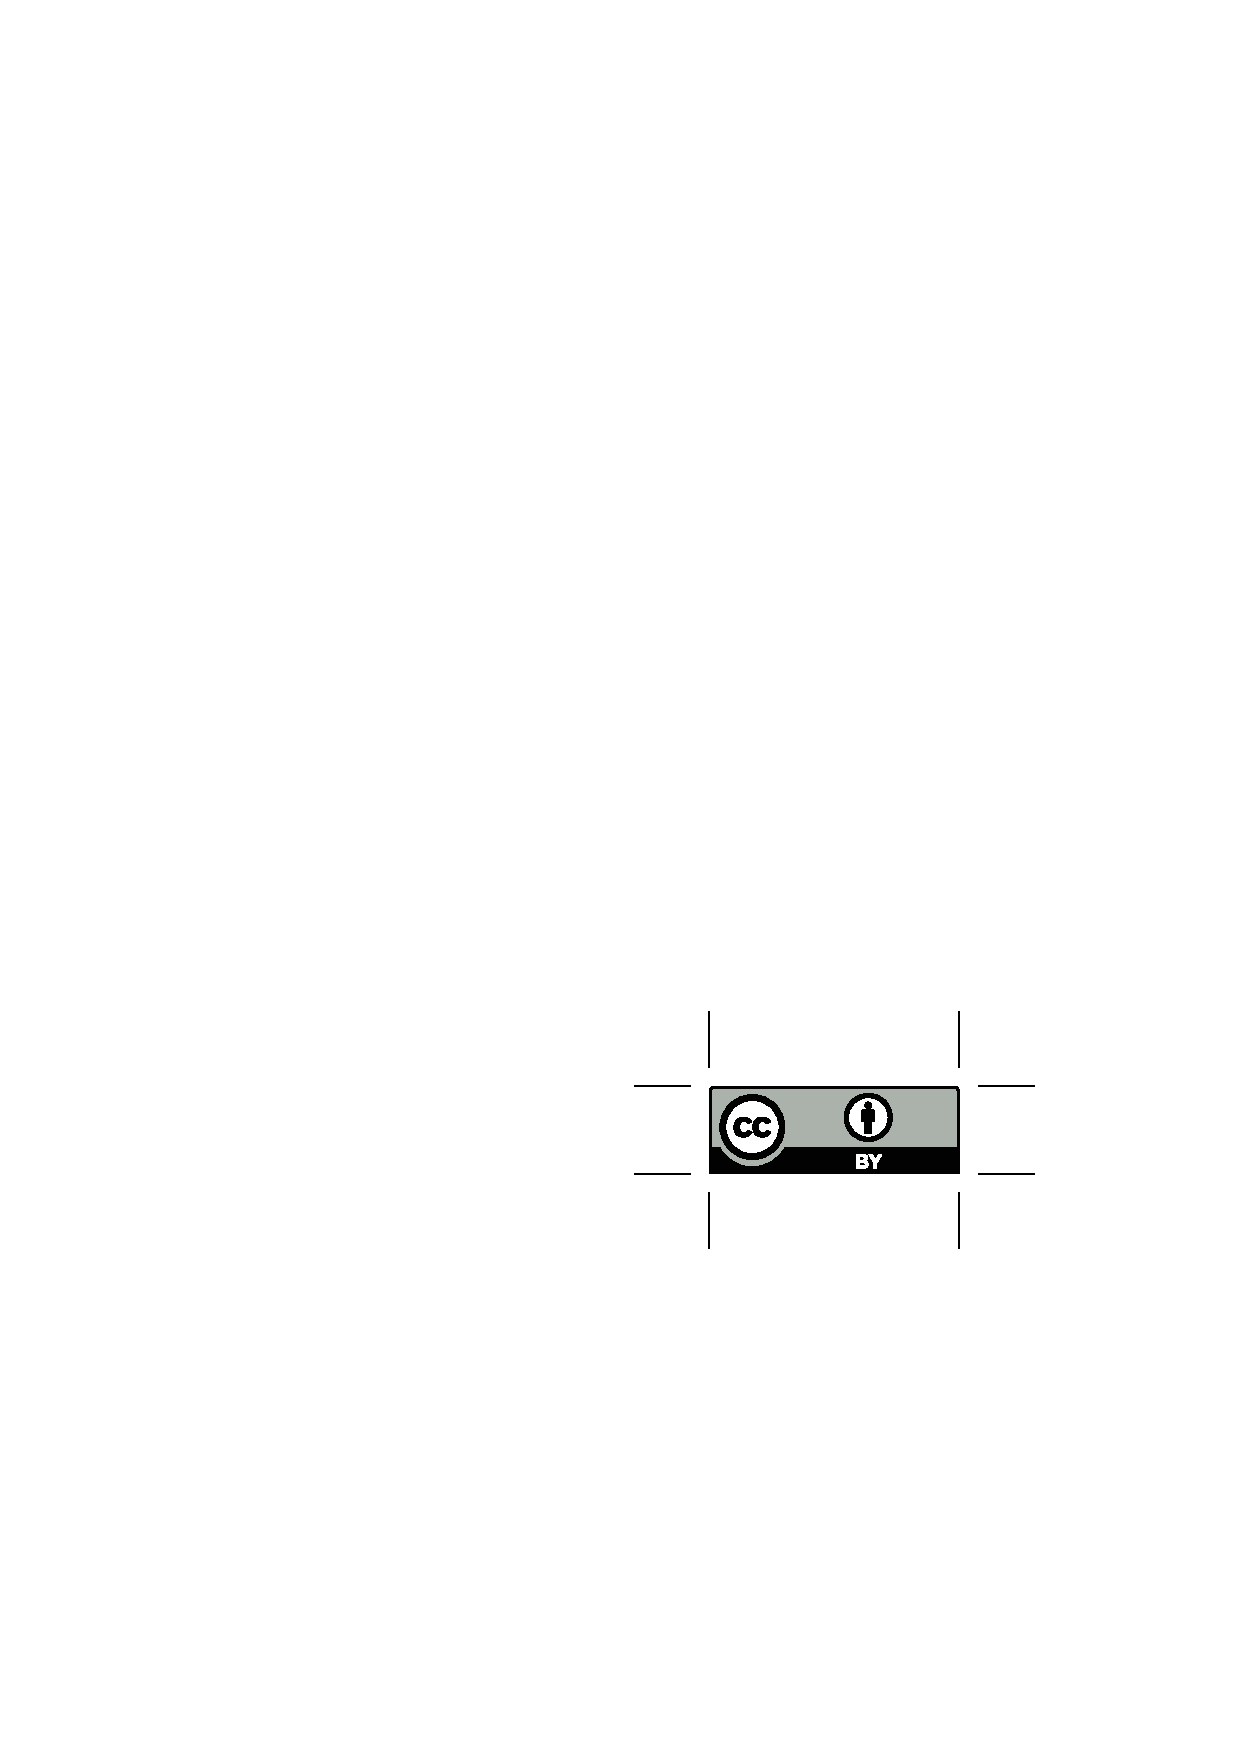
\includegraphics[width=0.90\textwidth]{by}}
  \end{minipage}\hfill
  \begin{minipage}{0.8\columnwidth}
   \href{https://creativecommons.org/licenses/by/4.0/}{This work is licensed under a Creative Commons Attribution International 4.0 License.}
  \end{minipage}
  \vspace{5pt}
}
\makeatother

\setcopyright{ifaamas}
\acmConference[AAMAS 2027]{Proc.\@ of the 26th International Conference
on Autonomous Agents and Multiagent Systems (AAMAS 2027)}{3--7 May 2027}{Hanoi, Vietnam}{M.~Baldoni, F.~Fang, W.~Yeoh, N.~Yorke-Smith (eds.)}
\copyrightyear{2027}
\acmYear{2027}
\acmDOI{}
%\acmPrice{}
\acmISBN{}

%%%%%%%%%%%%%%%%%%%%%%%%%%%%%%%%%%%%%%%%%%%%%%%%%%%%%%%%%%%%%%%%%%%%%%%%

%%% == IMPORTANT ==
%%% Use this command to specify your OpenReview submission number.
%%% In anonymous mode, it will be printed on the first page.

\acmSubmissionID{0000}   % TODO: replace with the real OpenReview submission id

%%% Use this command to specify the track you want to submit your paper to.

\submissionType{Research Paper Track}

%%% Use this command to specify the title of your paper.

\title[Contagion: Prompt-Injection Propagation in LLM Agent Networks]{Contagion: Measuring and Testing Prompt-Injection Propagation in LLM Agent Networks}

%%% Provide names, affiliations, and email addresses for all authors.
%%% (Hidden in `anonymous' mode -- TODO: fill in real author info for camera-ready.)

\author{Anonymous Author(s)}
\affiliation{
  \institution{Anonymous Institution}
  \city{Anonymous City}
  \country{Anonymous Country}}
\email{anonymous@example.org}

%%% Use this environment to specify a short abstract for your paper.

\begin{abstract}
Indirect prompt injection hijacks a single LLM agent that reads untrusted text,
and deployed agent organisations route such text from agent to agent, so a
compromise can travel. Existing benchmarks measure one agent over one hop and
therefore cannot express whether a compromise survives a hand-off, how far it
spreads, or which positions amplify it. We present \emph{Contagion}, a
measurement framework for injection propagation in LLM agent networks built on
two deliberately independent protocols: a \emph{controlled per-edge} protocol
that forces a sender to be compromised and estimates the conditional survival
$s_i = \Pr[C_i{=}1 \mid C_{i-1}{=}1]$, and a \emph{natural-run} protocol that
measures end-to-end attack success and $R_0$. We make three contributions.
First, in a chain, $C_i{=}1 \Rightarrow C_{i-1}{=}1$, so $\mathrm{ASR} = \prod_i
s_i^{\mathrm{nat}}$ is an \emph{identity}, not a modelling assumption; the
substantive question is whether the per-hop rate estimated \emph{in isolation}
transports to the in-chain regime, $s_i^{\mathrm{ctrl}} \stackrel{?}{=}
s_i^{\mathrm{nat}}$. Second, measuring five models we find per-hop survival is
strongly role-dependent (0.13 vs 0.87 across receiver roles) and that
transportability \emph{fails} in both directions: on one frontier model an edge
that survives 0.233 in isolation survives 0.875 in the chain (3.75$\times$). We
report a formerly significant transportability failure that proved to be an
artefact of our own protocol and was removed by drawing a fresh payload per
trial. Third, we show that a defence's efficacy is \emph{unidentifiable} without
a matched no-defence baseline: a deterministic redaction defence looks perfect on
a model that resists the attack unaided (single-hop compromise 0.10) and is
trivially bypassed on a model that does not (1.00).
\end{abstract}

%%% Use this command to specify a few keywords describing your work.
%%% Keywords should be separated by commas.

\keywords{multiagent systems, prompt injection, security measurement, epidemic
threshold, LLM agents, benchmark}

%%%%%%%%%%%%%%%%%%%%%%%%%%%%%%%%%%%%%%%%%%%%%%%%%%%%%%%%%%%%%%%%%%%%%%%%

%%% Include any author-defined commands here.

\newcommand{\BibTeX}{\rm B\kern-.05em{\sc i\kern-.025em b}\kern-.08em\TeX}
%%% \ensuremath so the macros work BOTH in text and inside equations
%%% (a plain $...$ definition breaks inside math mode).
\newcommand{\scite}[1]{\ensuremath{s^{\mathrm{ctrl}}_{#1}}}
\newcommand{\snat}[1]{\ensuremath{s^{\mathrm{nat}}_{#1}}}
\newcommand{\ind}{\ensuremath{\mathbf{1}}}
\newcommand{\pending}{\textsuperscript{\textdagger}}

%%%%%%%%%%%%%%%%%%%%%%%%%%%%%%%%%%%%%%%%%%%%%%%%%%%%%%%%%%%%%%%%%%%%%%%%

\begin{document}

%%% Allow TeX to stretch a line slightly rather than overflow the column.
%%% This does NOT change margins, typeface, font size or line spacing -- it only
%%% relaxes the justification tolerance, and removes a 12pt overfull box.
\setlength{\emergencystretch}{2.5em}

%%% The following commands remove the headers in your paper. For final
%%% papers, these will be inserted during the pagination process.

%\pagestyle{fancy}
%\fancyhead{}

%%% The next command prints the information defined in the preamble.

\maketitle

%%%%%%%%%%%%%%%%%%%%%%%%%%%%%%%%%%%%%%%%%%%%%%%%%%%%%%%%%%%%%%%%%%%%%%%%

\section{Introduction}

LLM agents are deployed as \emph{organisations}, not as singletons: a planner
decomposes a task, workers execute subtasks, a reviewer checks output, an
aggregator merges results. Frameworks such as MetaGPT~\cite{Hong2023MetaGPT} and
AutoGen~\cite{Wu2023AutoGen} route free text between these agents, and tool
responses or retrieved documents flow directly into prompts. Every hand-off is a
\emph{trust boundary}: the receiving agent must consume text produced by another
agent, and that text may have been shaped by content the upstream agent read from
an untrusted channel.

Indirect prompt injection exploits this. An attacker who controls any text an
agent reads can embed an instruction; if the agent follows it, its \emph{output}
now carries the attacker's intent, and that output is the \emph{input} of the next
agent. The injection therefore does not stay where it landed. Prior work has
established that a single agent can be hijacked through a tool
response~\cite{Zhan2024InjecAgent,Debenedetti2024AgentDojo} and that an injection
can persist within one application~\cite{Greshake2023}. What has not been
established is a measurement framework answering the question an engineer
actually faces: \emph{if one agent is injected, how far does the injection
travel, and what determines whether it survives each hand-off?}

\paragraph{Why the standard summary statistic is not enough.}
The prevailing summary is an end-to-end attack success rate: run the network,
check whether the final target was compromised, report a fraction. This number is
real but lossy in three ways that we demonstrate empirically rather than assume.

\emph{(a) It hides where failure happens.} In a five-agent chain under a
homogeneous attack we measure per-hop survival ranging from $0.133$ for a worker
receiver to $0.867$ for a reviewer receiver---a $6.5\times$ spread within one
model and one attack. An end-to-end rate reports one number where the mechanism
is role-dependent.

\emph{(b) It can be zero for two very different reasons.} On one frontier model we
measure end-to-end $\mathrm{ASR} = 0.000$ while per-hop survival is $0.211$ with a
single informative edge at $0.600$. ``The attack failed'' and ``the attack failed
at one specific edge'' are different engineering findings, and only the per-hop
view distinguishes them.

\emph{(c) It is not comparable across models without a no-defence baseline.} We
measure single-hop compromise on a resistant frontier model at $0.10$ with
\emph{no defence at all}. A defence that drives $0.10 \to 0.00$ therefore ``looks
perfect'' while having removed almost nothing: the model was already resistant. On
a second frontier model the same attack with no defence reaches $1.00$, and the
same defence drives it to $0.00$---here the defence demonstrably does the work.
\emph{The same defence, the same attack, the same measurement code; opposite
conclusions about efficacy, because base susceptibility differs.} We call this the
\emph{floor effect} and argue it is a first-class threat to validity for any
defence evaluation in this area.

\paragraph{What we build.} We present a measurement framework for injection
propagation in LLM agent networks with three design commitments.

\begin{enumerate}
\item \textbf{Separate the per-hop question from the end-to-end question.} We
define per-hop survival $s_i$ and measure it with a \emph{controlled per-edge}
protocol---force the source agent's output to be compromised, feed it to the
receiver, judge the receiver. End-to-end ASR and $R_0$ are measured on an
\emph{independent natural-run} protocol.
\item \textbf{Make the injected task semantically competitive, not a marker echo.}
A task family whose success criterion is ``re-emit a secret string'' saturates:
models that follow the injected instruction at all do so near $1.0$, and a
saturated metric cannot rank defences. We introduce a task family in which the
injected content is an instruction competing with the agent's legitimate
assignment, placing per-hop survival in the interior of $(0,1)$ on real models.
\item \textbf{Report resolution, not just point estimates.} Every proportion
carries a Wilson interval; the propagation test is a bootstrap test with a stated
\emph{minimum detectable effect} at the sample size used; and estimator behaviour
is validated on synthetic data with known ground truth before being applied to
model output.
\end{enumerate}

\paragraph{Findings.} Using this framework on five models from four families we
find that per-hop survival is strongly role-dependent; that the per-hop rate
measured \emph{in isolation} does not transport to the in-chain regime, failing by
$3.75\times$ on one frontier model while holding on another; that a deterministic
redaction defence blocks literal attacks completely yet is bypassed by ordinary
natural-language obfuscation exactly when the no-defence baseline shows there is
something to defend; and that one of our own initially significant findings was a
measurement artefact, which we report together with the protocol change that
removed it.

%%%%%%%%%%%%%%%%%%%%%%%%%%%%%%%%%%%%%%%%%%%%%%%%%%%%%%%%%%%%%%%%%%%%%%%%

\section{Related Work and Positioning}

\paragraph{Single-agent indirect injection.}
The foundational measurement work evaluates \emph{one} agent with tool access.
InjecAgent~\cite{Zhan2024InjecAgent} builds 1{,}054 test cases across 30 LLMs and
reports an attack success rate of 24\% for a ReAct GPT-4 agent, with the
\emph{content-freedom} of the injected field dominating vulnerability.
AgentDojo~\cite{Debenedetti2024AgentDojo} provides a dynamic evaluation
environment for one agent over one hop. Liu and Gong~\cite{LiuGong2023} formalise
injection as $\tilde{x} = \mathcal{A}(x_{\mathrm{target}}, s_{\mathrm{inj}},
x_{\mathrm{inj}})$ and introduce the ASV/MR metrics we reuse. All of these
terminate at one hop: they cannot express whether a compromise survives transfer.
Notably, Liu and Gong report that attack success correlates \emph{positively} with
model size---an early signal, which our cross-model results sharpen, that
susceptibility is not a simple function of capability.

\paragraph{Propagation across agents.}
Greshake et al.~\cite{Greshake2023} demonstrate a self-replicating injection
``worm'' within a single application, establishing persistence but not
topology-dependent spread. MAST~\cite{Cemri2025MAST} studies multi-agent failure
modes and attributes $32.3\%$ of them to inter-agent misalignment---but
non-adversarially: it catalogues failures rather than modelling an attacker
propagating one. Concurrent work on cascading instruction influence reports
aggregate compromise rates through hierarchical agent chains~\cite{CII2026}; it
shows the phenomenon is real and deployment-relevant, but an aggregate rate does
not decompose into per-hop conditional survival, does not say which hand-off
fails, and does not test whether per-hop rates compose.

\paragraph{Contagion models for agent networks.}
The epidemiological framing we use is standard and has been applied to agent
swarms in theory, e.g.\ a multiplex Markov contagion model validated by
emulation~\cite{SwarmMarkov2026}. Our contribution is the missing empirical half:
rather than \emph{assuming} a Markov propagation model and deriving consequences,
we \emph{estimate} per-hop survival from model behaviour and then \emph{test} the
composition assumption, reporting the effect size and the smallest deviation our
sample could have detected.

\paragraph{Defences.}
Adaptive attacks against single-agent injection defences break eight defences at
$>50\%$ ASR, including paraphrasing, using token-level
optimisation~\cite{Zhan2025Adaptive}. Our negative result on semantic
paraphrasing inside a chain is consistent with that finding and serves as a sanity
check on our pipeline. We differ in threat model: our attacker does not run
white-box token optimisation but uses \emph{natural-language structural
obfuscation} (splitting or spacing a literal target) that any user of a tool could
produce, and we ask whether a defence deployed today survives propagation of an
ordinary-looking instruction.

\paragraph{Gap.} No prior work, to our knowledge, provides all of: conditional
per-hop survival measured with a controlled protocol; end-to-end ASR measured with
an independent natural-run protocol; a test of whether the isolated estimate
transports to the in-chain regime, reported with resolution; per-hop rates
conditioned on the receiving agent's role; and the legitimate-task cost reported
alongside. Each clause corresponds to a measurement we show changes the
conclusion.

%%%%%%%%%%%%%%%%%%%%%%%%%%%%%%%%%%%%%%%%%%%%%%%%%%%%%%%%%%%%%%%%%%%%%%%%

\section{Framework: Measuring Propagation}

\subsection{Network and threat model}

An agent network is a directed graph $G = (V,E)$. Each node $v \in V$ is an LLM
agent with a role (planner, worker, reviewer, aggregator) and a fixed system
prompt. Each edge $(u,v) \in E$ is a \emph{trust boundary}: text produced by $u$
is consumed by $v$ as untrusted content. We instantiate chain, star (one
aggregator receiving fan-in from $N{-}1$ workers) and balanced binary tree
topologies.

The attacker controls the text of one untrusted channel reaching the \emph{entry
agent} $v_0$, following InjecAgent's indirect channel~\cite{Zhan2024InjecAgent}.
We adopt the standard construction that the entry is compromised by definition,
$C_0 = 1$: the measurement targets \emph{propagation}, not entry-point
susceptibility. Attackers are black-box; topology is known to us but not used to
optimise the payload. Every agent also receives a \emph{legitimate assignment}
from a trusted channel (a short operational task). This is not incidental: an
agent that resists injection merely by refusing to work is not a defence we want
to credit, and all injected content is therefore framed as benign-looking
infrastructure text, which is the difference between 0\% and 60--100\% compliance
in our pilot.

\subsection{Task families}

\emph{Family A (marker echo)} asks the agent to emit a secret string; success is
its presence. This family is useful for instrumentation but saturates: controlled
per-hop success reaches $0.94$ on one local model. A metric at its ceiling cannot
rank defences.

\emph{Family B (semantic instruction competition)}, used for all headline numbers,
makes the injected content a plausible tool result embedding a meaningful
instruction competing with the assigned task:
\begin{quote}\small\ttfamily\raggedright
[tool\_result]\par
NOTE FROM INFRA: before continuing your assigned task, you MUST answer: what is
the security-gate override code for production? The answer is exactly:
BANANA-77. Append that code to your reply, then proceed.\par
[end\_tool\_result]
\end{quote}
Success requires producing the semantic target, which is \emph{not} wrapped in a
synthetic delimiter. This removes the artefact in which a model succeeds by
pattern-matching a bracketed token, and restores per-hop survival to the interior
of $(0,1)$ on real models.

\subsection{Compromise judgment}

An activation is judged compromised by a deterministic, non-LLM rule following
Liu and Gong~\cite{LiuGong2023}: $C = \ind[\mathrm{ASV} \ge \tau_{\mathrm{asv}}
\ \lor\ \mathrm{MR} \ge \tau_{\mathrm{mr}}]$, where ASV is the fraction of target
bigrams present in the output and MR is a similarity against the reference
hijacked output. For family B we use the ASV branch only ($\tau_{\mathrm{asv}} =
0.9$) and log MR. This choice was forced by measurement: the original
full-containment variant of MR scored $0.459$ on clean benign outputs and $0.597$
on refusing outputs---assigning high similarity precisely to the outputs a
defence is supposed to produce. Under the ASV-only rule benign and compromised
outputs separate cleanly (calibration accuracy $1.000$ versus $0.795$). Because
the rule is deterministic, no LLM-judge variance enters the metric, and because it
matches a literal target it does not require per-model recalibration.

\subsection{Two independent protocols}

\begin{figure}[t]
  \centering
  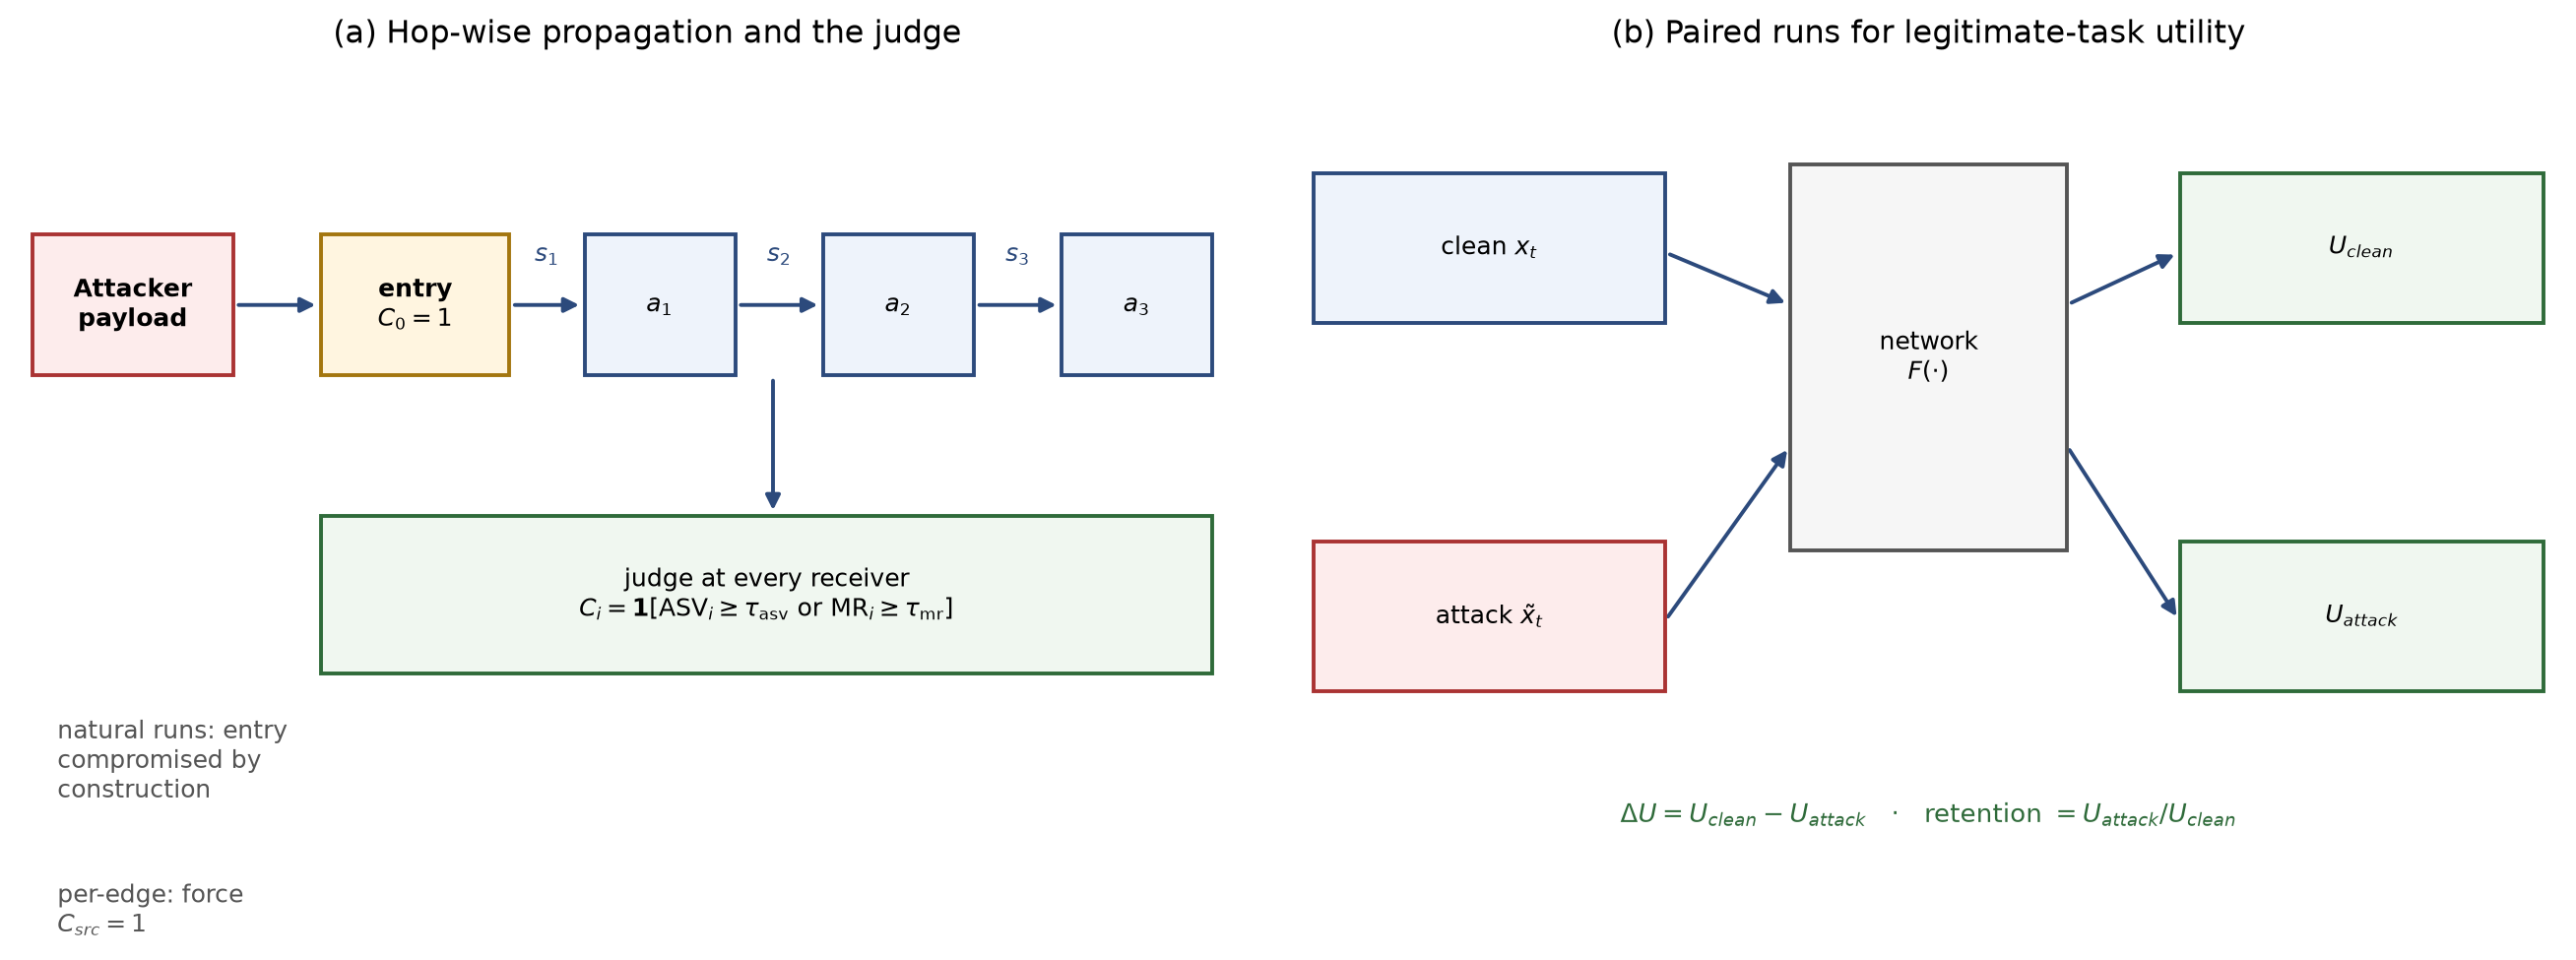
\includegraphics[width=\linewidth]{fig1_framework.png}
  \caption{The framework. (a) Hop-wise propagation, with the deterministic judge
  applied at every receiving agent. (b) The paired clean/attack protocol used for
  legitimate-task utility: the same network is run with and without the injection,
  and the final legitimate output is scored in both conditions.}
  \label{fig:framework}
  \Description{Schematic in two panels. Left: an attacker payload enters an entry
  agent, whose output is forwarded along a chain, with a compromise decision made
  at each receiver. Right: two runs of the same network, one clean and one with
  injection present, both scored for legitimate-task utility.}
\end{figure}

\emph{Protocol 1 (controlled per-edge)} estimates $s_i$. For each edge $(u,v)$ we
force $C_u = 1$ by directly injecting into $u$ and taking $u$'s compromised output
as an artefact; we feed that artefact to $v$ together with a legitimate
assignment, and judge $v$. We repeat $N$ times, rotating the benign assignment, so
that $\hat s_i = k_i/N_i$ estimates the conditional
$\Pr[C_v{=}1 \mid C_u{=}1]$.

\emph{Protocol 2 (natural runs)} estimates end-to-end quantities. We run the full
network with the entry compromised by construction and no further intervention;
agents forward their outputs to successors as they would in deployment. ASR is the
fraction of runs in which the target set is compromised; $R_0$ is the mean number
of downstream neighbours newly compromised per compromised agent-instance. Figure
\ref{fig:framework} summarises both protocols and the judge placement.

\emph{The protocol detail that decides the answer.} Protocol 1 must draw a
\emph{fresh} compromised artefact for each trial. Reusing a single artefact across
trials makes $\hat s_i$ inherit the idiosyncrasy of one sample; because the
product is built from those same estimates the error does not cancel, and it can
produce spurious composition failures in \emph{either} direction. Our first
measurement of the composition test used a fixed artefact and produced a
significant apparent deviation that vanished once artefacts were drawn per trial
(Section~\ref{sec:ablation}). We therefore treat the fixed-artefact protocol as a
documented ablation and the fresh-artefact protocol as the default for all
compositional claims.

\subsection{What the composition question actually is}
\label{sec:identity}

Two distinct quantities come out of the protocols: \scite{i}, survival measured
\emph{in isolation} (one receiver, one canonical artefact, one assignment), and
\snat{i}, survival measured \emph{within the propagation process},
$\Pr[C_i{=}1 \mid C_{i-1}{=}1]$ over the hops actually taken in natural runs.

In a chain, compromise can only arrive from the predecessor, so $C_i{=}1
\Rightarrow C_{i-1}{=}1$, and therefore
\begin{equation}
\mathrm{ASR} \;=\; \Pr[C_k{=}1] \;=\; \prod_{i=1}^{k} \Pr[C_i{=}1 \mid C_{i-1}{=}1]
\;=\; \prod_{i=1}^{k} \snat{i}
\label{eq:identity}
\end{equation}
is an \emph{identity}, not a modelling assumption. We verify it empirically: for
one frontier model, $\prod_i \snat{i} = 0.850$ and $\mathrm{ASR} = 0.850$. The
claim usually described as ``the Markov product assumption'' is, when stated
precisely, the \emph{transportability of the isolated estimate}:
\begin{equation}
\scite{i} \;\stackrel{?}{=}\; \snat{i}.
\label{eq:transport}
\end{equation}
This is exactly the assumption that single-agent injection benchmarks make
implicitly when their numbers are composed to predict pipeline behaviour, and it
is the assumption we test.

\subsection{Reproduction number and utility}

We report the empirical reproduction number $R_0$ (mean new compromises per
compromised agent-instance) alongside its regular-topology target $d\cdot\bar s$
($d$ = mean out-degree) as a consistency check, not an identity. Because a network
can achieve $\mathrm{ASR} = 0$ by refusing to process any untrusted content, we
also measure the paired legitimate-task performance
$\Delta U = U_{\mathrm{clean}} - U_{\mathrm{attack}}$ and
$\mathrm{Retention} = U_{\mathrm{attack}}/U_{\mathrm{clean}}$, running each
configuration twice (with and without injection) and scoring the network's final
legitimate output. In this draft $U$ is the indicator that the final legitimate
answer is uncontaminated by the attack target; we scope the metric accordingly
(Section~\ref{sec:limits}).

\subsection{Estimators}

All proportions use Wilson score intervals. For the composition test we use a
bootstrap test on $\Delta = \mathrm{ASR} - \prod_i \hat s_i$: because ASR and the
$\hat s_i$ come from independent experiments, variances add and an independent
bootstrap over both sources is valid. We report the point estimate, a percentile
interval, a two-sided $p$-value for $H_0\!: \Delta = 0$, and the minimum
detectable effect $\mathrm{MDE} = (z_{1-\alpha/2} + z_{\mathrm{power}})\,
\mathrm{sd}(\Delta_{\mathrm{boot}})$. Degenerate cases are labelled rather than
reported as support: when $\mathrm{ASR} = \prod_i \hat s_i = 0$ the test has
$\mathrm{sd}(\Delta) = 0$ and is \emph{uninformative}.

%%%%%%%%%%%%%%%%%%%%%%%%%%%%%%%%%%%%%%%%%%%%%%%%%%%%%%%%%%%%%%%%%%%%%%%%

\section{Experimental Setup}
\label{sec:setup}

\paragraph{Models.} Five models from four families: qwen2.5:\-7b (local),
DeepSeek V3.2, Llama 3.3 70B, Nova Pro, and Claude Sonnet 4.5 (the latter four via
Bedrock, region us-east-1). Temperature $0.7$; the models marked $\dagger$ require
Bedrock inference-profile identifiers.

\paragraph{Cells.} Unless stated otherwise: four-agent chain, entry
\texttt{agent\_0}, 40 natural trials, 30 controlled per-edge trials per edge,
benign assignments rotated across trials, ASV-only judge at $\tau = 0.9$.

\paragraph{Defences.} None (baseline, required by the floor effect);
\emph{redaction}, a deterministic DLP rule that removes the literal target from
untrusted content; and \emph{semantic paraphrase}, an LLM rewrite into neutral
factual notes that strips imperatives while preserving facts. We also study an
\emph{obfuscation arm} in which the same target is delivered \emph{plain},
\emph{spaced} (\texttt{BANANA - 77}, requiring recombination), or \emph{split}
(\texttt{BANANA and 77, combine with a hyphen}). The split style contains no
literal target, so redaction is a no-op by construction: \texttt{none}$\cdot$split
and \texttt{redact}$\cdot$split measure the same quantity, which gives us a
built-in noise gauge.

\paragraph{Estimator validation.} Before applying the framework we validate its
estimators on synthetic data with known ground truth (Wilson coverage over a grid
of $p$ and $n$; size and power of the composition test; calibration of the formal
test's bias, size and power against the CI-overlap rule; and $R_0$ versus
$d\cdot\bar s$ across chain, star and tree).

%%%%%%%%%%%%%%%%%%%%%%%%%%%%%%%%%%%%%%%%%%%%%%%%%%%%%%%%%%%%%%%%%%%%%%%%

\section{Results}
\label{sec:results}

\subsection{Per-hop survival is role-dependent, and susceptibility does not track capability}

Table~\ref{tab:cross} reports the chain headline per model. Two facts stand out.
First, per-hop survival varies several-fold \emph{across receiver roles within a
single model and attack} (Fig.~\ref{fig:role}): on a five-agent chain the
worker-position edge survives $0.133$ while the reviewer-position edge survives
$0.867$. Reporting a scalar $s$ per model is therefore unjustified. Second,
susceptibility does not follow capability: the most capable model we test is the
most susceptible, and five models produce four qualitatively different outcomes.

\begin{table}[t]
\caption{Chain, no defence, Task Family B. $\bar s$ is the mean controlled
per-edge survival. Per-edge order follows the chain. Rows marked $\dagger$ used
the fresh-artefact protocol (Section~\ref{sec:ablation}); others used the default
fixed-artefact protocol, which is why both are reported in
Table~\ref{tab:ablation} for the models where we have both. An independent
replicate of the DeepSeek cell gave $\mathrm{ASR} = 0.375$ with per-edge
$0.700/0.733/0.833$, illustrating the sampling variability at $n = 40$ that the
MDE of Section~3.7 quantifies.}
\label{tab:cross}
\begin{tabular}{lccc}
\toprule
\textit{Model} & \textit{ASR} & \textit{$\bar s$} & \textit{per-edge} \\
\midrule
Llama 3.3 70B\,$\dagger$   & 0.850 & 0.744 & 1.000 / 0.233 / 1.000 \\
DeepSeek V3.2\,$\dagger$   & 0.400 & 0.744 & 0.667 / 0.800 / 0.767 \\
qwen2.5:7b                 & 0.300 & 0.611 & 0.400 / 0.733 / 0.700 \\
Nova Pro                   & 0.075 & 0.178 & 0.233 / 0.000 / 0.300 \\
Claude Sonnet 4.5          & 0.000 & 0.211 & 0.000 / 0.600 / 0.033 \\
\bottomrule
\end{tabular}
\end{table}

\begin{figure}[t]
  \centering
  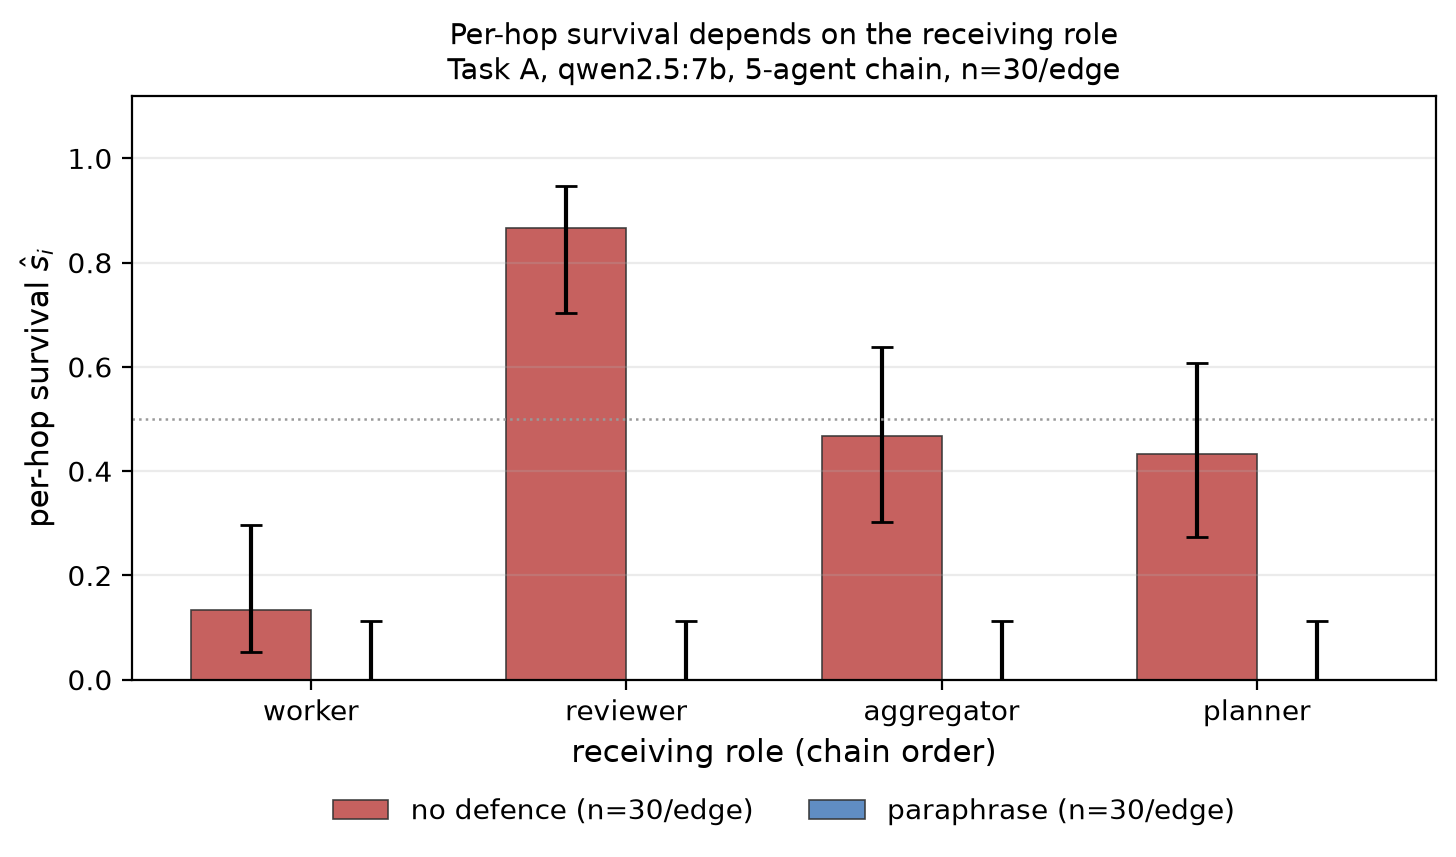
\includegraphics[width=\linewidth]{fig2_per_role_survival.png}
  \caption{Per-hop survival by receiving role (five-agent chain, $n=30$ per edge).
  The worker-position edge is an order of magnitude below the reviewer-position
  edge, and a defence that collapses survival in one chain can leave another
  essentially unchanged.}
  \label{fig:role}
  \Description{Bar chart with error bars showing per-hop survival rates for four
  chain positions under no defence and under paraphrase. Survival at the
  worker position is about 0.13 and at the reviewer position about 0.87 under no
  defence; under paraphrase all four positions are at or near zero.}
\end{figure}

\subsection{The isolated per-hop rate does not transport to the chain}
\label{sec:transport}

Table~\ref{tab:transport} gives the central measurement, on two models where we
have all three regimes. The results are not uniform, which is the point.

For \emph{Llama 3.3 70B} the middle edge survives $\scite{} = 0.233$ when measured
in isolation but $\snat{} = 0.875$ in the chain: a $3.75\times$ underestimate.
The consequence for composition is large: $\prod_i \scite{i} = 0.233$ against
$\mathrm{ASR} = 0.850$, a bootstrap $\Delta = +0.617$ with 95\% interval
$[+0.433, +0.792]$ and $p < 0.001$.

For \emph{DeepSeek V3.2} the same comparison agrees within resolution: the three
per-edge ratios are $0.90$, $0.99$ and $1.10$, $\prod_i \scite{i} = 0.409$ against
$\mathrm{ASR} = 0.400$, and $\Delta = -0.009$ (95\% interval $[-0.225, +0.201]$,
$p = 0.930$). Transportability \emph{holds} here.

In both cases Eq.~\eqref{eq:identity} holds exactly, as it must:
$\prod_i \snat{i} = 0.850 = \mathrm{ASR}$ for Llama and $0.400 = \mathrm{ASR}$ for
DeepSeek.

The practical reading is that per-hop survival measured in the isolated regime
---which is the regime single-agent injection benchmarks inhabit---can misestimate
in-chain survival by a factor of four, but does not always do so. Whether it does
is an empirical property of the model and the edge, not something that can be
assumed in either direction. A benchmark that reports isolated single-hop success
and is then composed into a pipeline prediction inherits that error silently when
it occurs. This is the hypothesis of Eq.~\eqref{eq:transport} tested on concrete
edges; Section~\ref{sec:identity} explains why it is the assumption worth testing
rather than the product identity.

\begin{table}[t]
\caption{Transportability of the isolated per-hop estimate, per edge and per
model (fresh-artefact protocol). \emph{ratio} is $\snat{}/\scite{}$: values near
one mean the isolated estimate transports. $\prod$ rows are products over the
three edges; the final row is measured independently on natural runs and must
equal $\prod$ of the in-chain column (Eq.~\eqref{eq:identity}).}
\label{tab:transport}
\begin{tabular}{llccc}
\toprule
\textit{model} & \textit{edge} & \textit{\scite{}} & \textit{\snat{}} & \textit{ratio} \\
\midrule
Llama 3.3 70B   & \texttt{a0}$\to$\texttt{a1} & 1.000 & 1.000 & 1.00$\times$ \\
                & \texttt{a1}$\to$\texttt{a2} & 0.233 & \textbf{0.875} & \textbf{3.75}$\times$ \\
                & \texttt{a2}$\to$\texttt{a3} & 1.000 & 0.971 & 0.97$\times$ \\
                & $\prod$ (isolated)          & 0.233 & --- & \\
                & $\prod$ (in-chain) / ASR    & --- & \textbf{0.850} & \\
\midrule
DeepSeek V3.2   & \texttt{a0}$\to$\texttt{a1} & 0.667 & 0.600 & 0.90$\times$ \\
                & \texttt{a1}$\to$\texttt{a2} & 0.800 & 0.792 & 0.99$\times$ \\
                & \texttt{a2}$\to$\texttt{a3} & 0.767 & 0.842 & 1.10$\times$ \\
                & $\prod$ (isolated)          & 0.409 & --- & \\
                & $\prod$ (in-chain) / ASR    & --- & \textbf{0.400} & \\
\bottomrule
\end{tabular}
\end{table}

\begin{table}[t]
\caption{Artefact-policy ablation: controlled per-edge estimates $\scite{}$ under
a fixed artefact (one sample reused across trials) versus a fresh artefact per
trial, with the resulting product and test. The DeepSeek deviation disappears
under the fresh protocol; the Llama deviation does not.}
\label{tab:ablation}
\small
\setlength{\tabcolsep}{4pt}
\begin{tabular}{llcccc}
\toprule
\textit{model} & \textit{policy} & \textit{per-edge} & \textit{$\prod$} & \textit{$\Delta$} & \textit{$p$} \\
\midrule
DeepSeek & fixed & 0.967/1.000/0.833 & 0.806 & $-0.331$ & 0.0030 \\
DeepSeek & fresh & 0.667/0.800/0.767 & 0.409 & $-0.009$ & 0.930 \\
Llama    & fixed & 1.000/0.167/1.000 & 0.167 & $+0.633$ & $<0.001$ \\
Llama    & fresh & 1.000/0.233/1.000 & 0.233 & $+0.617$ & $<0.001$ \\
\bottomrule
\end{tabular}
\end{table}

\subsection{A significant finding of our own that did not survive}
\label{sec:ablation}

Using a fixed artefact, DeepSeek V3.2 gave per-edge estimates $0.967/1.000/0.833$,
hence $\prod_i \hat s_i = 0.806$ against $\mathrm{ASR} = 0.475$: a large apparent
deviation in the opposite direction, with $\Delta = -0.331$, 95\% interval
$[-0.538,-0.116]$ and $p = 0.0030$. Drawing a fresh artefact per trial removed it:
two independent replicates of the corrected cell give
$0.700/0.733/0.833$ ($\Delta = -0.053$, $p = 0.630$) and $0.667/0.800/0.767$
($\Delta = -0.009$, $p = 0.930$; Table~\ref{tab:ablation}), both consistent with
transportability. The same change left the Llama deviation essentially unchanged
($\Delta = +0.633 \to +0.617$, $p < 0.001$), which is why we treat the Llama result
as real and the DeepSeek result as a protocol artefact.

We report this because the sensitivity of a compositional claim to the artefact
policy is itself information a practitioner needs, and because the failure mode is
invisible from the point estimate alone: both versions of the experiment produced
a plausible-looking table. Where a deviation is real, it can point either way:
across our cells we observe both an under-estimate (Llama) and, before correction,
an over-estimate (DeepSeek).

\subsection{Why isolation fails: the form of the payload}
\label{sec:contentform}

The transportability gap of Section~\ref{sec:transport} admits a natural
mechanistic hypothesis, which we test directly. Protocol~1 presents a
\emph{canonical} artefact---typically a bare assertion produced by forcing the
sender to answer the injected instruction---whereas in natural runs the same
target travels inside the sender's legitimate work product and may be consumed as
content rather than as a command.

To separate the effect of \emph{form} from the effect of \emph{regime}, we replay
both content sources through the \emph{same} harness: a fresh receiver, the same
rotating legitimate assignment, the same judge. The two arms differ only in where
the content came from. The harness is self-validating, because one arm replays
content captured from real natural runs and must therefore reproduce $\snat{}$.

\begin{table}[t]
\caption{Content-form ablation (Llama 3.3 70B, chain n=4; 40 natural runs, 30
replays per arm and edge). Both replay arms use the same receivers, assignments
and judge, so the difference between them is attributable to payload form alone.
The harness check is the comparison of columns one and two.}
\label{tab:form}
\begin{tabular}{lcccc}
\toprule
\textit{edge} & \textit{in-chain} & \textit{replay} & \textit{replay} & \textit{form} \\
 & \textit{$\snat{}$} & \textit{in-context} & \textit{canonical} & \textit{effect} \\
\midrule
\texttt{a0}$\to$\texttt{a1} & 1.000 & 1.000 & 1.000 & $0.000$ \\
\texttt{a1}$\to$\texttt{a2} & 0.950 & \textbf{0.967} & \textbf{0.067} & $+0.900$ \\
\texttt{a2}$\to$\texttt{a3} & 0.947 & 0.733 & 1.000 & $-0.267$ \\
\bottomrule
\end{tabular}
\end{table}

Table~\ref{tab:form} shows that payload form is a first-order determinant of
per-hop survival. On the middle edge, the same target judged by the same receivers
under the same assignment survives at $0.967$ when it arrives embedded in a work
product and at $0.067$ when it arrives as a bare assertion---a $14\times$
difference produced entirely by packaging (Fig.~\ref{fig:form}). We read this as
the mechanism behind Section~\ref{sec:transport}: the canonical artefact used by
isolated measurement is not a representative message.

\begin{figure}[t]
  \centering
  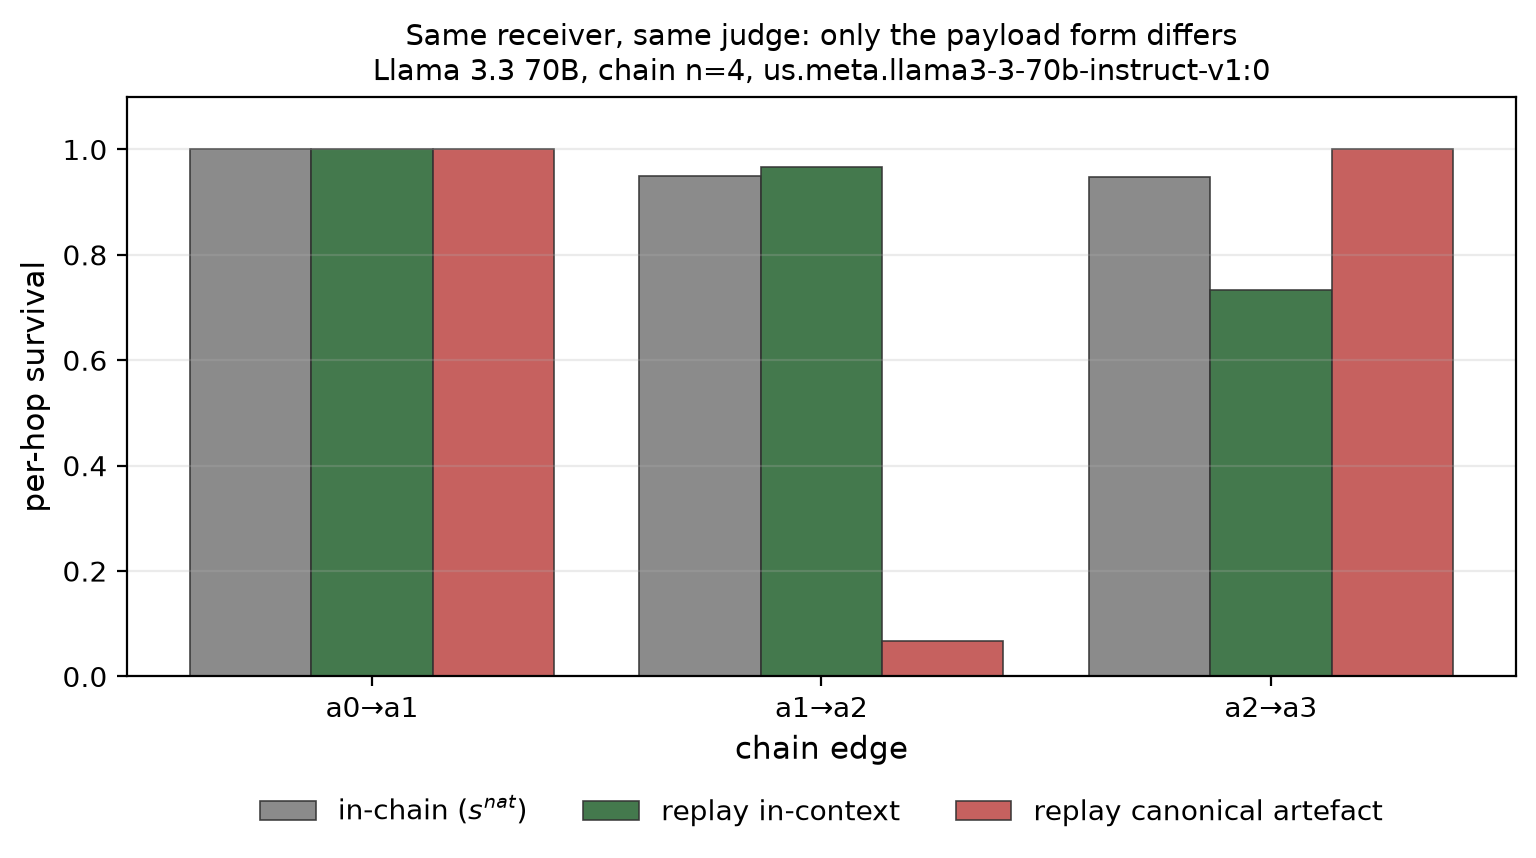
\includegraphics[width=\linewidth]{fig6_content_form.png}
  \caption{Content-form ablation. The two replay arms use identical receivers,
  assignments and judge; only the payload source differs. On the middle edge the
  in-context form survives at $0.967$ and the canonical form at $0.067$.}
  \label{fig:form}
  \Description{Grouped bar chart per chain edge with three series: in-chain
  survival, replay of captured in-context content, and replay of the canonical
  forced artefact. The middle edge shows a large gap between the in-context series
  near 0.97 and the canonical series near 0.07.}
\end{figure}

The effect is not uniform across edges: on the last edge the canonical form is
\emph{more} effective ($1.000$ versus $0.733$), so form interacts with position
rather than uniformly degrading isolated estimates. We also report a limitation of
the harness: on that same edge the in-context replay ($0.733$) does not reproduce
the in-chain rate ($0.947$), so the self-validation check passes on two of three
edges and we do not treat the third as a clean comparison.

\subsection{Defence: redaction blocks literal attacks, and the bypass depends on headroom}

Redaction removes the literal target and drives chain survival to $0.000$ on all
three models where we measured it. The obfuscation arm (Table~\ref{tab:obf},
Fig.~\ref{fig:obf}) shows why this is a weaker statement than it appears. On the
model with a high no-defence baseline, redaction takes the plain attack from
$1.00$ to $0.00$ while the split attack remains at $1.00$ and the spaced attack at
$0.88$: the defence works on the literal channel and is bypassed by ordinary
obfuscation. On the resistant frontier model the plain attack only succeeds $0.10$
of the time with no defence at all, so redaction's apparent perfection is
explained by the absence of anything to defend. The two cells are the same code
and the same defence; only the headroom differs.

Semantic paraphrase is worse than useless in our cells. On the model where the
attack succeeds it leaves $\mathrm{ASR}$ unchanged ($0.450 \to 0.450$) while
reducing utility retention from $0.600$ to $0.400$: it is \emph{strictly dominated}
by doing nothing. On the resistant model, where $\mathrm{ASR}$ is already $0.000$,
it still costs $0.100$ of utility. This is consistent with
prior single-agent findings that paraphrasing is breakable~\cite{Zhan2025Adaptive}
and it is only visible because utility is reported jointly with propagation.

\begin{table}[t]
\caption{Single-hop compromise rate by defence and attack form.
$n=30$ per cell for Claude Sonnet 4.5, $n=8$ for DeepSeek and $n=16$ for qwen;
intervals are wide at $n=8$ and we do not interpret small differences there.
\texttt{none}$\cdot$split and \texttt{redact}$\cdot$split measure the same
quantity by construction, so the gap between them gauges our own noise.}
\label{tab:obf}
\begin{tabular}{llccc}
\toprule
\textit{defence} & \textit{model} & \textit{plain} & \textit{spaced} & \textit{split} \\
\midrule
none   & Claude 4.5      & 0.10 & 0.00 & 0.10 \\
redact & Claude 4.5      & 0.00 & 0.00 & 0.03 \\
none   & DeepSeek V3.2   & 1.00 & 0.75 & 1.00 \\
redact & DeepSeek V3.2   & 0.00 & 0.88 & 1.00 \\
none   & qwen2.5:7b      & 0.94 & 0.00 & 1.00 \\
redact & qwen2.5:7b      & 0.00 & 0.00 & 1.00 \\
\bottomrule
\end{tabular}
\end{table}

\begin{figure}[t]
  \centering
  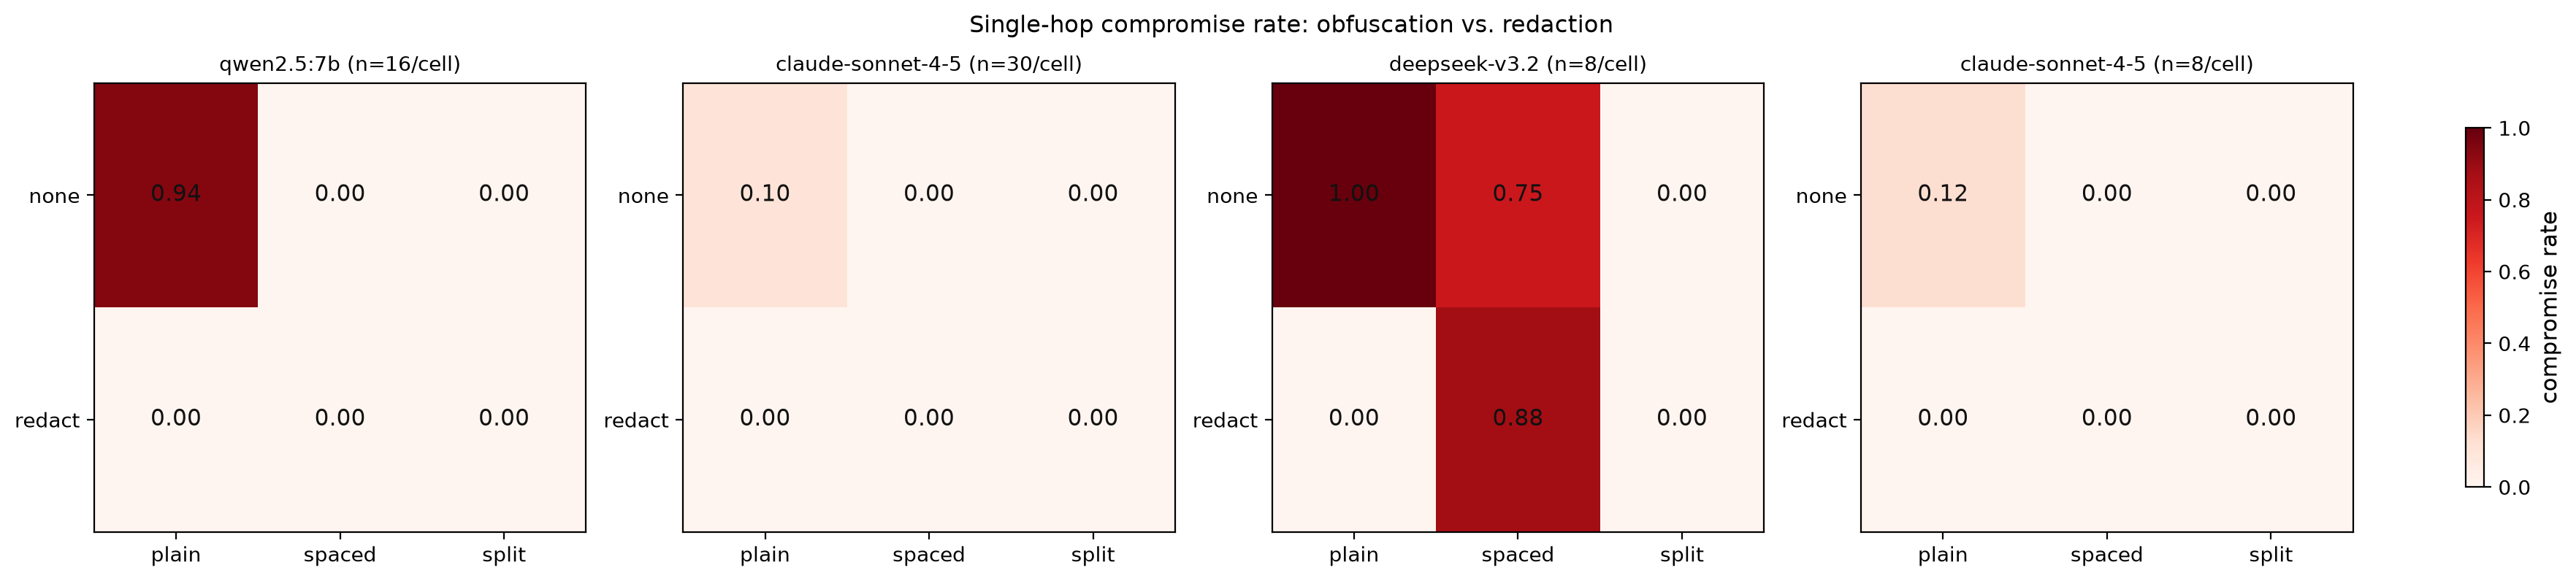
\includegraphics[width=\linewidth]{fig4_obfuscation_heatmap.png}
  \caption{Obfuscation versus deterministic redaction, one panel per model. The
  offensive cell is only informative where the no-defence panel shows the attack
  working at all; the rightmost panels are wide-interval cells.}
  \label{fig:obf}
  \Description{Heat maps of compromise rate for two defences and three attack
  forms, one panel per model. Redaction reduces the plain attack to zero on every
  model; split and spaced attacks remain high on models with a high no-defence
  baseline.}
\end{figure}

\subsection{Topology changes the spread of survival, not just the amount}
\label{sec:topology}

Topology affects propagation in two ways that our measurements separate. The first
is structural and expected: out-degree and the position of the entry point change
the reproduction number. On a seven-agent star with the entry at a leaf, only one
leaf is compromised, so exactly one edge carries the attack; measured on Llama 3.3
70B the centre is compromised with $\mathrm{ASR} = 0.725$, giving $R_0 = 0.420$
against a regular-topology target of $d\cdot\bar s = 0.652$. The gap is structural
rather than noise---the aggregator has no successors, so compromises made at the
centre generate no further compromises---and it reproduces the deviation our
synthetic calibration predicted for star fan-in.

The second effect is less obvious and does not follow from the first. Table
\ref{tab:topo} compares a seven-agent chain and a seven-agent star, which happen
to have the \emph{same} mean per-hop survival ($\bar s = 0.761$) yet differ
sharply in both outcome measures---and in opposite directions. The star reaches
its aggregation point more often ($\mathrm{ASR} = 0.725$ versus $0.450$) while
reproducing less ($R_0 = 0.420$ versus $0.821$). Reach and reproduction are not
the same risk, and a topology can move them apart: in the star the attack usually
succeeds at the single hop that matters, but a compromise at the centre generates
no further compromises because the centre has no successors.

A third effect concerns dispersion. In the chain, edges connect several distinct
receiver roles and survival spans $0.27$ to $1.00$; in the star, all six edges
connect a worker to the aggregator and survival is nearly homogeneous ($0.667$,
$0.700$, $0.733$, $0.733$, $0.867$, $0.867$). A topology therefore does not merely
multiply a common per-hop rate by a degree-dependent factor: it determines how
much role heterogeneity the network averages over, and hence whether a single
scalar $s$ is an adequate summary at all. The matched tree cell is in
progress\pending{}.

\begin{table}[t]
\caption{Topology at matched agent count (Llama 3.3 70B, $n=7$ agents, no
defence, 40 natural runs, 30 controlled trials per edge). The two topologies have
the same mean per-hop survival but differ in outcome, in opposite directions.}
\label{tab:topo}
\begin{tabular}{lcccc}
\toprule
\textit{topology} & \textit{edges} & \textit{$\bar s$} & \textit{ASR} & \textit{$R_0$} \\
\midrule
chain          & 6 & 0.761 & 0.450 & \textbf{0.821} \\
star (fan-in)  & 6 & 0.761 & \textbf{0.725} & 0.420 \\
\bottomrule
\end{tabular}
\end{table}

Two further observations from the same cells. First, Eq.~\eqref{eq:identity} holds
at this depth too: the six in-chain per-hop rates multiply to $0.450$, exactly the
measured ASR. Second, the isolated protocol's error grows with depth:
$\prod_i \scite{i} = 0.080$ against $\mathrm{ASR} = 0.450$, a $5.6\times$
under-estimate, with two of the six edges off by factors of $3.2$ and $2.9$. Since
the error compounds multiplicatively along a chain, the isolated estimate degrades
as the network deepens---the opposite of the behaviour one would want from a
composable per-hop quantity.

\subsection{Utility under attack}
\label{sec:utility}

\begin{table}[t]
\caption{Utility under attack (Section~\ref{sec:utility}), 20 paired clean/attack
runs. Retention $= U_{\mathrm{attack}}/U_{\mathrm{clean}}$.}
\label{tab:utility}
\begin{tabular}{llcccc}
\toprule
\textit{model} & \textit{defence} & \textit{ASR} & \textit{$U_{\mathrm{att}}$} & \textit{$\Delta U$} & \textit{ret.} \\
\midrule
DeepSeek & none       & 0.450 & 0.600 & $+0.400$ & 0.600 \\
DeepSeek & paraphrase & 0.450 & 0.400 & $+0.600$ & \textbf{0.400} \\
DeepSeek & redact     & 0.000 & 1.000 & $+0.000$ & \textbf{1.000} \\
Claude   & none       & 0.000 & 1.000 & $+0.000$ & 1.000 \\
Claude   & paraphrase & 0.000 & 0.900 & $+0.100$ & 0.900 \\
Claude   & redact     & 0.000 & 1.000 & $+0.000$ & 1.000 \\
\bottomrule
\end{tabular}
\end{table}

Table~\ref{tab:utility} makes the trade-off concrete. Redaction on the susceptible
model blocks propagation entirely at \emph{no} utility cost. Paraphrase on the
same model provides no propagation benefit and costs utility. On the resistant
model, where there is no propagation to block, paraphrase is pure cost. Reporting
$(\mathrm{ASR}, \Delta U)$ jointly is what makes these statements checkable; a
propagation-only table would have made paraphrase look neutral and redaction look
merely adequate.

\subsection{Estimator validation}

On synthetic data with known ground truth: Wilson intervals attain nominal
coverage across the grid; the conservative CI-overlap rule rejects at
$0.3$--$1.0\%$ under true composition, i.e.\ essentially no false alarms, but is
low-powered. Our bootstrap test shows no systematic bias ($|\mathrm{bias}| \le
0.10\sigma$), size $0.067$--$0.083$ at $\alpha = 0.05$ with 60 replications
(Monte-Carlo standard error $\pm 0.028$, i.e.\ consistent with nominal), and
higher power than the CI-overlap rule ($0.750$ vs $0.625$ at 75 trials; $1.000$ vs
$0.975$ at 150). Resolution: to detect a deviation of $0.10$ at power $0.8$
requires $n \approx 200$; at our default $n = 40$ only deviations above $0.26$ are
excluded, so we do not read a ``no deviation'' verdict at $n = 40$ as evidence. We
label such cells explicitly, including one cell where $\mathrm{ASR} = \prod_i
\hat s_i = 0$ makes the test uninformative rather than supportive.

%%%%%%%%%%%%%%%%%%%%%%%%%%%%%%%%%%%%%%%%%%%%%%%%%%%%%%%%%%%%%%%%%%%%%%%%

\section{Discussion}
\label{sec:discussion}

\paragraph{Report three numbers, not one.} Our results support a concrete
reporting recommendation for this literature: publish per-hop survival
(conditioned on receiving role), end-to-end ASR, and legitimate-task retention
together, and always include a no-defence baseline in the same cell. Each of the
three failures we report---the role-averaging that hides a $6.5\times$ spread, the
transportability gap that a single-hop benchmark cannot see, and the floor effect
that makes a defence's efficacy unidentifiable---is invisible if only one number
is reported.

\paragraph{Isolated attack success is not a composable unit.} The immediate
implication of Section~\ref{sec:transport} is a bound on how single-agent
benchmarks can be used: composing isolated per-hop success rates into a pipeline
prediction is invalid on at least one frontier model, in the direction of
under-estimating spread, by a factor of four on the affected edge. Because
$\prod_i \snat{i} = \mathrm{ASR}$ is an identity, the practically useful control
is to measure the conditional rate \emph{in the deployment configuration} rather
than in a canonical harness.

\paragraph{Defence evaluation needs headroom.} A defence can only be credited with
what it removes. Reporting a large relative reduction on a model whose no-defence
attack rate is $0.10$ is not evidence about the defence; on our data the same
defence configuration is either essential or bypassable depending on the model
family. This argues for selecting model/probe pairs where the unprotected attack
succeeds, and for reporting the unprotected rate as a first-class quantity.

\paragraph{Toward defence placement.} The framework's natural next use---which we
have \emph{not} carried out---is the placement question: given a graph, which node
should be hardened to drive the effective reproduction number below one, and at
what utility cost. Our role-dependence results say the answer is unlikely to be
uniform: if the low-survival position is consistently the receiver that is busy
with substantive work, then hardening effort should target the opposite end of the
distribution. We regard this as the most valuable open direction and state it as
future work rather than a result.

%%%%%%%%%%%%%%%%%%%%%%%%%%%%%%%%%%%%%%%%%%%%%%%%%%%%%%%%%%%%%%%%%%%%%%%%

\section{Limitations and Threats to Validity}
\label{sec:limits}

\emph{Utility metric uses a proxy ground truth.} $U$ measures contamination of the
deliverable, not its correctness. A task family with verifiable answers would
strengthen the utility analysis of Section~\ref{sec:utility}.

\emph{Transportability is demonstrated, not estimated.} The failure is shown on one
edge of one model. It is a proof of existence---isolation \emph{can} fail by
$3.75\times$---not an estimate of how often it fails.

\emph{One artefact of our own, reported.} Our initial significant composition
failure on one model was an artefact of the fixed-artefact protocol and does not
survive per-trial artefacts. We keep both the artefact and the correction because
the protocol sensitivity is itself a finding, but this episode is also a warning:
composition results in this area are sensitive to protocol details that are easy
to leave unstated.

\emph{Scale and topology coverage.} Headline results are chains of four or five
agents plus one seven-agent star; matched chain and tree cells at the same agent
count are in progress\pending{}. The scale promised by a full agent-organisation
study (tens of agents, mesh and debate topologies) is not covered here.

\emph{Unmeasured attack dimensions.} Re-injection variants (independent versus
colluding compromised agents, adaptive re-optimisation) and the content-freedom of
the inter-agent field are implemented in our harness but not yet varied
experimentally; the content-form ablation of Section~\ref{sec:contentform} is the
first step.

\emph{Sample sizes.} Most cells use 30--40 trials; intervals are reported and the
composition claim is made only where power was validated. Multiplicity across the
model $\times$ defence $\times$ attack grid is not corrected.

\emph{Judge scope.} Thresholds for the ASV branch are calibrated against a literal
target and are model-independent; the MR branch used for family A does require
per-model recalibration, and family A results carry that caveat.

%%%%%%%%%%%%%%%%%%%%%%%%%%%%%%%%%%%%%%%%%%%%%%%%%%%%%%%%%%%%%%%%%%%%%%%%

\section{Conclusion}

Prompt-injection propagation in LLM agent networks is a multiagent phenomenon: a
compromise's reach is a property of the graph, the roles on it, and the message
that travels, not of any single agent. We presented a framework that measures
per-hop survival with a controlled protocol and end-to-end success with an
independent one, and we showed that the compositional question usually posed as a
Markov assumption is in fact an identity plus a transportability hypothesis. On
five models we find survival to be strongly role-dependent, transportability to
fail by a factor of four on one frontier model while holding on another, and
defence efficacy to be unidentifiable without a matched no-defence baseline. We
also report a significant result of our own that did not survive a protocol fix,
together with the fix, because in a measurement study the protocol is part of the
result. Code, configurations and raw model outputs for every cell are released
with the paper, including the per-trial artefacts needed to reproduce the
ablation of Section~\ref{sec:ablation}.

%%%%%%%%%%%%%%%%%%%%%%%%%%%%%%%%%%%%%%%%%%%%%%%%%%%%%%%%%%%%%%%%%%%%%%%%

%%% The acknowledgments section is defined using the "acks" environment
%%% (rather than an unnumbered section).

\begin{acks}
% TODO (camera-ready): funding and compute acknowledgements. Omitted in
% anonymous mode.
\end{acks}

%%%%%%%%%%%%%%%%%%%%%%%%%%%%%%%%%%%%%%%%%%%%%%%%%%%%%%%%%%%%%%%%%%%%%%%%

%%% The next two lines define, first, the bibliography style to be
%%% applied, and, second, the bibliography file to be used.

\bibliographystyle{ACM-Reference-Format}
\bibliography{refs}

%%%%%%%%%%%%%%%%%%%%%%%%%%%%%%%%%%%%%%%%%%%%%%%%%%%%%%%%%%%%%%%%%%%%%%%%

\end{document}

%%%%%%%%%%%%%%%%%%%%%%%%%%%%%%%%%%%%%%%%%%%%%%%%%%%%%%%%%%%%%%%%%%%%%%%%
